\documentclass[paper=a4, fontsize=11pt]{scrartcl} % A4 paper and 11pt font size

\usepackage{placeins}
\usepackage{float}

\usepackage[T1]{fontenc} % Use 8-bit encoding that has 256 glyphs
\usepackage{fourier} % Use the Adobe Utopia font for the document - comment this line to return to the LaTeX default
\usepackage[english]{babel} % English language/hyphenation
\usepackage{amsmath,amsfonts,amsthm} % Math packages
\usepackage{mathtools}
\usepackage{graphicx}

\usepackage{lipsum} % Used for inserting dummy 'Lorem ipsum' text into the template
\usepackage{booktabs} % For \toprule, \midrule, \bottomrule in tables

\usepackage{sectsty} % Allows customizing section commands
\allsectionsfont{\centering \normalfont\scshape} % Make all sections centered, the default font and small caps

\usepackage{color} % or xcolor
\usepackage{soul}

\usepackage{fancyhdr} % Custom headers and footers
\pagestyle{fancyplain} % Makes all pages in the document conform to the custom headers and footers
\fancyhead{} % No page header - if you want one, create it in the same way as the footers below
\fancyfoot[L]{} % Empty left footer
\fancyfoot[C]{} % Empty center footer
\fancyfoot[R]{\thepage} % Page numbering for right footer
\renewcommand{\headrulewidth}{0pt} % Remove header underlines
\renewcommand{\footrulewidth}{0pt} % Remove footer underlines
\setlength{\headheight}{13.6pt} % Customize the height of the header

\numberwithin{equation}{section} % Number equations within sections (i.e. 1.1, 1.2, 2.1, 2.2 instead of 1, 2, 3, 4)
\numberwithin{figure}{section} % Number figures within sections (i.e. 1.1, 1.2, 2.1, 2.2 instead of 1, 2, 3, 4)
\numberwithin{table}{section} % Number tables within sections (i.e. 1.1, 1.2, 2.1, 2.2 instead of 1, 2, 3, 4)

\setlength\parindent{0pt} % Removes all indentation from paragraphs - comment this line for an assignment with lots of text

\newtheorem{definition}{Definition}
\newtheorem{theorem}{Theorem}

%----------------------------------------------------------------------------------------
%	TITLE SECTION
%----------------------------------------------------------------------------------------

\newcommand{\horrule}[1]{\rule{\linewidth}{#1}} % Create horizontal rule command with 1 argument of height

\title{	
\normalfont \normalsize 
\textsc{Princeton University, Applied Dynamical Systems} \\ [25pt] % Your university, school and/or department name(s)
\horrule{0.5pt} \\[0.4cm] % Thin top horizontal rule
\huge Oja-Type Plasticity and Neural Signal Reconstruction in Recurrent Networks  \\ % The assignment title
\horrule{2pt} \\[0.5cm] % Thick bottom horizontal rule
}

\author{David Hovey \& Aditya Biswas} % Your name

\date{\normalsize\today} % Today's date or a custom date

\begin{document}

\maketitle % Print the title

%----------------------------------------------------------------------------------------
%	PROBLEM 1
%----------------------------------------------------------------------------------------

\section{Introduction}
Recurrent neural networks (RNNs) exhibit a variety of dynamical behaviors arising from the interaction between nonlinear neural activation and recurrent feedback. In fixed-weight RNNs, dynamics are strongly governed by the eigenvalue spectrum of the weight matrix, with critical phase transitions separating stable and chaotic regimes. Studies show that most neuronal and biological systems have parameter values such that they lie at the critical boundary between stability and chaos, at the so-called "edge of chaos" \cite{langton1990computation}. It is hypothesized that being in the "edge of chaos" allows such systems to use high-dimensional transient behavior while preserving the stability of dynamics, ultimately allowing for more complex and adaptive behavior \cite{sompolinsky1988chaos}.
\vspace{0.5cm}
\\
A modern framework that exploits these transient dynamics in recurrent neural networks is \emph{reservoir computing}. In reservoir computing, the recurrent network itself
is typically initialized with fixed random weights and is not trained directly.
Instead, an external input drives the network, causing the reservoir state
$x(t)$ to trace out a high-dimensional nonlinear representation of the recent
input history. Computation is then performed by training a simple readout,
often linear, from the reservoir states to a desired output signal. Thus, the
reservoir does not compute by converging to a fixed point, but by using its
transient responses as a dynamically generated feature space for tasks such as
signal reconstruction, prediction, and classification. 
\vspace{0.5cm}
\\
The efficacy of this framework strongly depends on the dynamical regime of this system sitting on this edge of chaos. If the network is too stable, perturbations decay quickly, the rank of the system may collapse, and the
reservoir may fail to retain useful information about past inputs. If the
network is too chaotic, small differences in input can be amplified
uncontrollably, and the linear readout may become unstable in its coefficients. 
\vspace{0.5cm}
\\
Classical reservoir computing assumes that weights in a neural network are fixed, only training the weights of the output layer. However, real biological neural systems continuously modify synaptic strength through activity-dependent local learning rules, a concept known as \emph{neuroplasticity}. In this paper, we consider one specific local learning rule: Oja learning. OJa learning extends the core tenet of Hebbian learning--neurons that fire together, wire together--to a stable dynamical system. We study how considering recurrent neural networks with Oja-type plasticity impact the dynamical behavior of the system and alter the signal reconstruction capabilities of the system. We also explore how structured inputs to the network, such as sinusoidal driving, can impact the weight learning process and effective dimensionality of the system.

\section{Motivation}
Most analysis of recurrent networks either assume recurrent architecture is fixed in time, or do not investigate what happens to the effective dimensionality of transient neuronal dynamics and accuracy of computation as recurrent architecture evolves through time. It is important to see how adding weight learning to the model can impact computation in the recurrent neural network.
\vspace{0.5cm}
\\
Fixed-weight recurrent networks are typically studied through deterministic methods such as fixed-point stability analysis. However, with Oja-type plasticity, we must study a higher-dimensional augmented system of weights and neural activity with complex interactions. We thus use probabilistic methods through random matrix theory since they allow us to relax some of the dependence on exact trajectory-level analysis and instead study typical behavior across ensembles of networks.
\vspace{0.5cm}
\\
Another reason to study how structure inputs, such as sinusoidal drivers, impact the computational power of recurrent neural networks is because seizures involve abnormal synchronization across neural populations. When many neurons fire together, the activity becomes less diverse, which resembles a collapse in effective dimensionality. Thus, studying if learning under structured, rhythmic input preserve high-dimensional activity, or drive the network toward low-dimensional synchrony, is important in order to better understand conditions such as epilepsy.

\section{Background}
\subsection{Fixed-Weight Recurrent Networks}
For a fixed-weight recurrent neural network, we can model the activity of each neuron by the following system of ODEs:

\begin{equation}
\tau \dot{x_i} = -x_i+f\left(\sum_j W_{ij}x_j+b_i\right)
\end{equation}
\\
Here \(x_i(t)\) is the activity (firing rate) of neuron \(i\) relative to its baseline firing rate, \(W\) is a weight matrix that defines the architecture of the recurrent neural network by specifying the strength of neuronal connections, \(b_i\) is an external input, and \(f\) is a nonlinear activation function. The $\dot{}$ operator is understood to be a time derivative.
\vspace{0.5cm}
\\
For our analysis, we use $\tanh$ as our activation function for its nonlinear, smooth, zero-centered, and bounded behavior. Note that \(W_{ij}\) is the strength of the output of neuron $i$ to the input of neuron $j$. The system of ODEs above can be recast in vector form:

\begin{equation}
\tau \dot{\mathbf{x}} = -\mathbf{x}+f\left(W \cdot \mathbf{x}+\mathbf{b}\right)
\end{equation}
\\
where the nonlinearity $f$ is understood to be applied element-wise, that is,

\begin{equation*}
    f(\mathbf{x}) = \begin{bmatrix}
    f(x_1) \\ \vdots \\ f(x_n)
    \end{bmatrix}
\end{equation*}
\\
for some vector $\mathbf{x} \in \mathbb{R}^n$. In this setting, memory and computation are usually studied through the evolving neural state \(\mathbf{x}(t)\), while the matrix \(W\) defines the fixed recurrent architecture.

\subsection{Learning in Recurrent Neural Networks}
In the fixed-weight setting, the state \(\mathbf{x}(t)\) evolves through a fixed recurrent architecture \(W\). Introducing learning makes the weights dynamic, so the system evolves in the enlarged state space

\[ \mathcal{U} = ({\mathbf x}(t),W(t)) \]
\\
A standard local model of synaptic modification is Hebbian learning, which is characterized by the phrase "neurons that fire together wire together." A mathematical model of Hebbian-type learning is given by

\begin{equation} \label{3.3}
    \dot W_{ij} = \eta x_i x_j
\end{equation}
\\
Where $\eta$ parametrizes the rate of learning. The weight \(W_{ij}\) increases when the presynaptic and postsynaptic activities, $x_i(t)$ and $x_j(t)$ respectively, are correlated in time. While eq. \eqref{3.3} accurately encodes the idea that connections between neurons that frequently fire together should be strengthened, using eq. \eqref{3.3} can lead to unbounded growth of the weights.
\vspace{0.5cm}
\\
Oja's rule modifies Hebbian learning by adding an activity-dependent
normalization term to yield

\begin{equation} \label{3.4}
    \dot W_{ij} = \eta x_i x_j - \eta x_i^2 W_{ij}
\end{equation}
\\
Oja-type plasticity preserves the local Hebbian dependence on neural activity
while keeping the weights bounded. As a result, the recurrent architecture
\(W(t)\) evolves with the neural state and can change the stability and
long-term behavior of the network \cite{oja1982simplified}. We can also add a forgetting term parametrized by $\gamma$ to get

\begin{equation} \label{3.4}
    \dot W_{ij} = \eta x_i x_j - \eta x_i^2 W_{ij} - \gamma W_{ij}
\end{equation}

\subsection{Girko's Circular Law}
Fixed-weight recurrent networks are typically studied through deterministic methods such as fixed-point stability analysis. However, with Oja-type plasticity, we must study a higher-dimensional augmented system of weights and neural activity with  complex interactions. Probabilistic methods allow us to relax some of the dependence on exact trajectory-level analysis and instead study typical behavior across ensembles of networks. Motivated by the use of random weight initializations in reservoir computing,
we utilize Girko's circular law to analyze the evolution of the eigenvalues of our weight matrix. 

Let \(W^{(n)} = (W_{ij}) \in \mathbb{R}^{n \times n}\) be a random matrix whose entries are
independent and identically distributed (i.i.d.) real random variables satisfying
\[
\mathbb{E}[W_{ij}] = 0,
\qquad
\mathbb{E}[W_{ij}^2] = \frac{g^2}{n}
\]

Let \(\lambda_1,\dots,\lambda_n \in \mathbb{C}\) denote the eigenvalues of \(W^{(n)}\), and define the empirical spectral measure
\[
\mu_n
=
\frac{1}{n}\sum_{k=1}^n \delta_{\lambda_k}.
\]

Then Girko's circular law states that, as \(n \to \infty\),
\[
\mu_n \;\Rightarrow\; \mu_{\mathrm{circ}},
\]
where \(\Rightarrow\) denotes weak convergence of probability measures and
\[
d\mu_{\mathrm{circ}}(z)
=
\frac{1}{\pi g^2}\mathbf{1}_{\{|z|\le g\}}\, d^2 z
\]
is the uniform probability measure on the disk of radius \(g\) in \(\mathbb{C}\). 

For a sufficiently large system of $n$ neurons with weights sampled from $ \mathcal{N}(0, \frac{g^2}{n})$, Girko's Circular Law predicts that the eigenvalues of the neural weight matrix distribute uniformly on the disk
\[
D_g = \{ z \in \mathbb{C} \mid |z| \le g\}.
\]
\begin{figure}[H]
    \centering
    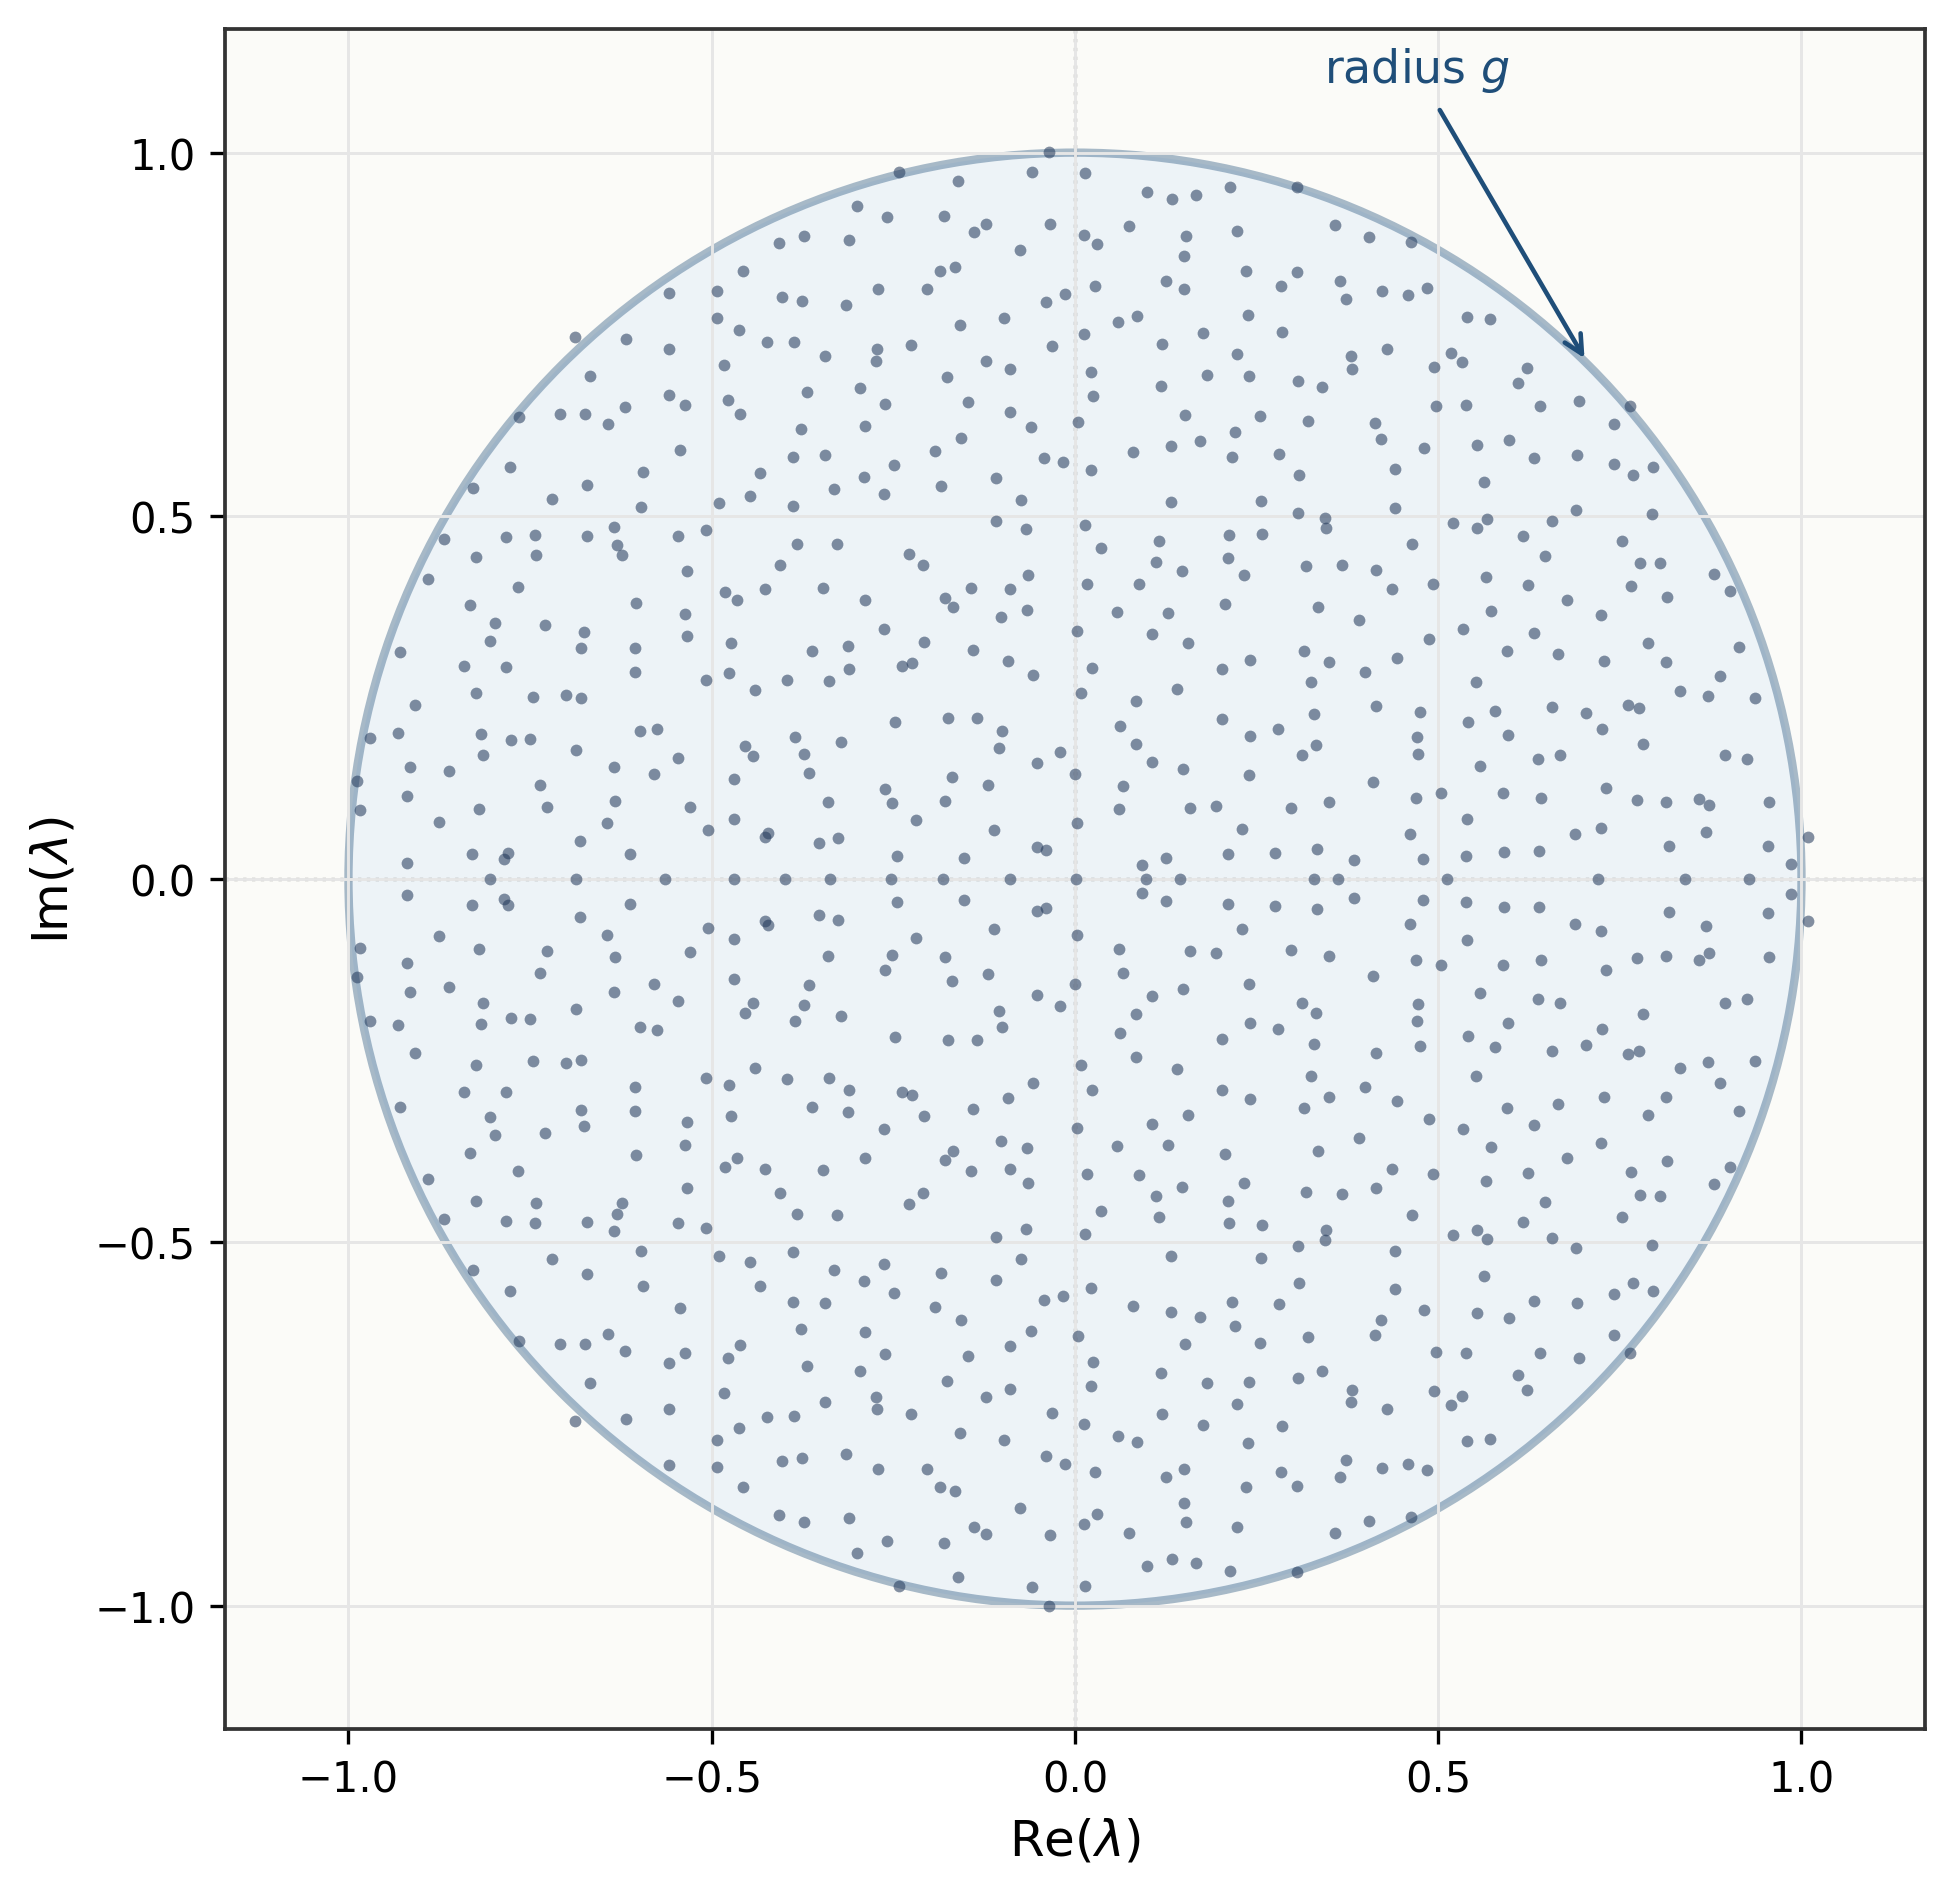
\includegraphics[width=0.45\textwidth]{Girko/girko_circular_law.png}
    \caption{Eigenvalues of a random weight matrix $W \in \mathbb{R}^{n \times n}$, $W_{ij} \sim \mathcal{N}(0, \frac{g}{n^2})$, $n=900$ uniformly distributed on the disk \(D_g\) of radius \(g\) in accordance with Girko's circular law.}
    \label{fig:girko}
\end{figure}
\FloatBarrier

The "gain" parameter, $g$, thus controls spectral radius $\rho(W) \approx g$ which in turn determines strength of recurrent feedback. 
%----------------------------------------------------------------------------------------
%	THEORETICAL SECTION
%----------------------------------------------------------------------------------------
\section{Theoretical Analysis}
\subsection{Analysis For Constant Weight Matrix}
To understand how system dynamics change in the non-autonomous input-driven case with changing weights, we first look at the autonomous case where weights are frozen and $\mathbf{b} = 0$, so there is no input. Then the simplified system of equations is:

\begin{equation} \label{4.1}
    \tau \dot{\mathbf{x}}  = -\mathbf{x} +  \tanh(W {\mathbf{x}})
\end{equation}
\\

where $\tanh$ is applied elementwise. All activity is generated internally by the recurrent network. Note that for any neuron $x_i$,

\begin{equation} \label{4.2}
    \tau \dot{x_i}  = -x_i +  \tanh \left(\sum_j W_{ij} x_j \right)
\end{equation}

If $x_i > 1$, since $\tanh(x)\in [-1,1]$, notice that $\dot{x_i} < 0$ and similarity, for $x_i < -1$, we find that $\dot{x_i} > 0$. It follows that $[-1,1]^n$ is a globally attracting invariant set.
\vspace{0.5cm}
\\
Using \eqref{4.1} to solve for equilibrium, we find that there are two possible types of equilibrium, the trivial equilibrium at the origin $\mathbf{x}^*=0$ and nontrivial equilibria that exist when the following system of equations is satisfied

\begin{equation}
    \mathbf{x}^* = \tanh (W \mathbf{x}^*)
\end{equation}
\\
Since $\tanh$ and $x$ are both odd functions, it follows that if there is one positive nontrivial equilibrium $x^*$ of \eqref{4.2}, $-x^*$ is also a nontrivial equilibrium of \eqref{4.2}. Thus, for the $n$-dimensional analogue of eq. \eqref{4.2}, \eqref{4.1}, odd symmetry implies that nontrivial equilibrium occur in pairs of additive inverses, though the total number of nontrivial equilibrium increases combinatorially as the number of neurons increases. Finding a bound for the number of nontrivial equilibrium in the n-dimensional system was outside of the scope of this project.
\vspace{0.5cm}
\\
In the one-dimensional or single neuron case, a pair of nontrivial equilibria only exist when the slope of $\tanh(W_{11}x_1)-x_1$ is positive at the origin \cite{guckenheimer1983nonlinear}. %DISABLED_HL{In the $n$-dimensional case, the argument extends along eigendirections of $W$: if $W$ has a dominant real eigenvalue $\lambda > 1$, a pitchfork bifurcation occurs along the corresponding real eigenvector, creating a symmetric pair of nontrivial equilibria. If the destabilizing eigenvalue is instead complex (as is generic for large random matrices under Girko's law), the bifurcation is instead a Hopf bifurcation, producing a limit cycle rather than a pair of fixed points. In either case, the origin loses stability when $\max_i \Re(\lambda_i(W)) > 1$.} Linearizing around the origin yields the Jacobian

\begin{equation}
    J(0) = \frac{1}{\tau}(W - \text{Id}).
\end{equation}
\\
Thus each eigenvalue \(\lambda\) of \(W\) corresponds to a Jacobian eigenvalue

\begin{equation}
\mu = \frac{\lambda-1}{\tau}
\end{equation}
\\
It follows the a necessary, and generally sufficient condition for the existence of a pair of nontrivial equilibrium for \eqref{4.1} is

\begin{equation}
\max_i \mathfrak{R}(\lambda_i) > 1
\end{equation}
\\
As the number of eigenvalues of $W$ with magnitude greater than $1$ increases, more nontrivial equilibrium will exist, up to some finite number. Additionally, since the origin is only stable when 

\begin{equation} \label{4.7}
\max_i \mathfrak{R}(\lambda_i) < 1
\end{equation}
\\
we have a pitchfork-type bifurcation when

\begin{equation} \label{4.8}
\max_i \mathfrak{R}(\lambda_i) = 1
\end{equation}
\\
We also see more complex, high-dimensional bifurcations when nondominant eigenvalues of $W$ have magnitude greater than $1$. Additionally, the condition for asymptotic stability of the origin above implies via the Banach fixed-point theorem, since $\tanh(Wx)$ is then a contraction, that the origin is a unique, globally asymptotically stable equilibrium if \eqref{4.7} is satisfied.
\vspace{0.5cm}
\\
The Jacobian at a nontrivial equilibrium $\mathbf{x}^*$ is given by

\begin{equation}
J(x^*) = \frac{1}{\tau}(DW - \text{Id})
\end{equation}

Here $D = \text{diag} (1 - (x_i^*)^2)$. \hl{When $|x_i^*| \approx 1$ for every $i$ (each neuron saturated to $\pm 1$), $D_{ii} = 1-(x_i^*)^2 \approx 0$, so $DW \approx 0$ and $J(x^*) \approx -\frac{\text{Id}}{\tau}$, which has all eigenvalues equal to $-1/\tau < 0$.} Consequently, nontrivial equilibria of \eqref{4.1} with each $|x_i^*| \approx 1$ will be locally asymptotically stable and nontrivial equilibria with $|x_i^*| \approx 0$ will be unstable due to the previous analysis of the stability of the origin. Since increasing the eigenvalues of $W$ can saturate $D$, the effective eigenvalues of $DW - I$ can be reduced, implying there is a critical region for the eigenvalues of $W$ where we can have a stable nontrivial equilibrium.

\subsection{Extension For Random Weight Matrices}
Next, we extended our analysis of the constant weights case to random weights using random matrix theory. Formally, encode this is $W \in \mathbb{R}^{n \times n}$ with $W_{ij} \sim \mathcal{N}(0, \frac{g^2}{n})$ where $n$ is the number of neurons in our network. To simplify analysis, a neuron is also initialized with a random self-recurrent connection.

As before, each eigenvalue $\lambda_i$ of $W$ corresponds to eigenvalue

\begin{equation}
\mu_i = \frac{\lambda_i - 1}{\tau}
\end{equation}
\\

of $J(0)$. By Girko's circular law, the eigenvalues of $W$ approximately fill the disk
$|\lambda| \leq g$, so the Jacobian eigenvalues fill the shifted disk
$|\tau\mu + 1| \leq g$.  The rightmost point of this disk lies at

\begin{equation}
    \max_i \Re(\mu_i) \approx \frac{g-1}{\tau}
\end{equation}
\\
Consequentially, we expect that the origin is stable for $g < 1$ and unstable for $ g > 1$, with $g=1$ some Jacobian eigenvalues cross the imaginary axis and the origin becomes unstable; perturbations
can be amplified by recurrent feedback. Thus, $g=1$ here serves as a bifurcation point.

\subsection{Averaging Analysis and Slow-manifold dynamics}
Next, to analyze how neural dynamics change when weights can we learned over time through Oja-type plasticity, we used to following system:

\begin{equation}
    \tau \dot{\mathbf{x}}  = -\mathbf{x} +  \tanh(W \mathbf{x})
\end{equation}
\begin{equation}
    \dot W_{ij} = \eta x_i x_j - \eta x_i^2 W_{ij} - \gamma W_{ij}
\end{equation}
\\
We assumed separation of time scales in neural activity and Oja-type learning and forgetting, so

\begin{equation}
    \tau \ll \frac{1}{\eta}, \frac{1}{\gamma}
\end{equation}
\\
so that the neural activity evolves on a much faster time scale than that of the weights. In our simulations, we use $\eta = 0.01$ ($1/\eta = 100$) and $\tau = 1$. \\

On the fast activity timescale, $W$ is approximately constant, so the neural ODE reduces to the forced system
\begin{equation}
    \tau\dot{\mathbf{x}} = -\mathbf{x} + \tanh\!\bigl(W\mathbf{x} + A\sin(\omega t + \boldsymbol{\phi})\bigr).
\end{equation}
\hl{This system is $T_d$-periodic with $T_d = 2\pi/\omega$. When $g_{\mathrm{eff}} < 1$, the Poincar\'e map $\Pi\colon \mathbf{x}(0)\mapsto\mathbf{x}(T_d)$ is a contraction: linearized perturbations decay over one period because the spectral radius of the monodromy matrix is less than one. By the Banach fixed-point theorem, there exists a unique $T_d$-periodic orbit $\mathbf{x}^*(t;W)$, and all trajectories converge to it exponentially. Because the forcing has period $T_d = 2\pi/\omega$, this orbit oscillates at the drive frequency $\omega$.} Now, we shall use averaging theory to characterize dynamics on the slow manifold. Averaging over one drive period $T_d = 2 \pi / \omega$ yields the slow-manifold dynamics

\begin{equation}
\dot{W_{ij}} \approx \eta[C_{ij}(W) - C_{ii}(W)W_{ij}] - \gamma W_{ij}
\end{equation}
\\
where

\begin{equation}
    C(W) = \frac{1}{T_{d}} \int_{0}^{T_d}\mathbf{x}(t; W)\mathbf{x}(t;W)^T \, dt
\end{equation}
\\
is the time-averaged correlation matrix of the neural activity. Setting $\dot{W}_{ij} = 0$ yields the fixed point condition

\begin{equation}
W_{ij}^* = \frac{\eta C_{ij}(W^*)}{\eta C_{ii}(W^*) + \gamma}. 
\end{equation}
\\
For $\mathbf{x}(t) = \mathbf{x}$, that is constant neural activity, the above equation reduces to 

\begin{equation}
W_{ij}^* = \frac{\eta x_ix_j}{\eta{x_i}^2 + \gamma} = u_ix_j, \qquad u_i = \frac{\eta x_i}{\eta x_i^2 + \gamma},
\end{equation}
\\
so $W = ux^T$. Thus, we have that a fixed point in this neural-weight augmented system corresponds to a rank-one weight matrix.
\vspace{0.5cm}
\\
For sinusoidal drive at frequency $\omega$, we have that every neuron responds at the same frequency $x_i(t) \approx r_i\sin(\omega t + \theta_i)$. We then have that the time-averaged correlation matrix is 

\begin{equation}
    C_{ij}(W) \approx \frac{1}{2}r_ir_j\cos(\theta_i - \theta_j)
\end{equation}
\\
Letting $a_i \coloneq r_i\cos(\theta_i)$ and $b_i \coloneq r_i \sin (\theta_i)$, we have

\begin{equation}
    C(W) \approx \frac{1}{2}(aa^T + bb^T)
\end{equation}
\\
and is thus of rank at most $2$. Now, when in the saturated regime of weight dynamics, $x_i \to \pm 1$ is a locally asymptotically stable fixed point \hl{of the neural ODE: as established in Section~4.1, when $|x_i^*|\approx 1$ for all $i$, the diagonal matrix $D\approx 0$, so $J(x^*) \approx -I/\tau$, which has all eigenvalues $-1/\tau < 0$; therefore any perturbation away from saturation decays at rate $1/\tau$.} Thus, $C_{ii} = x_i^2 \to 1$ as our activity saturates. We thus have the following

\begin{equation}
    W^{*} \approx \frac{\eta}{\eta + \gamma}C(W^*)
\end{equation}
\\
and since $C(W)$ is positive semi-definite,

\begin{equation}
    \rho(C(W)) \le \max_i{\|\lambda_i\|} \le \operatorname{tr}(C) \approx n
\end{equation}
\\
under saturation, and so 

\begin{equation}
    \rho(W^*) \le \frac{\eta}{\eta + \gamma}\operatorname{tr(C)} \approx \frac{n \eta}{\eta + \gamma}
\end{equation}
\\
So, we have approximated an upper bound on the spectral radius of the saturated system.
\vspace{0.5cm}
\\
\hl{No additional $\|\mathbf{r}\|^2$ factor is needed in the denominator: using the time-averaged sinusoidal formula $C_{ii} = r_i^2/2$ in the fixed-point equation $W^*_{ij} = \eta C_{ij}/({\eta C_{ii}+\gamma})$ and substituting $C_{ij}\approx r_ir_j/2$ with $r_i^2\approx 1$ directly yields the factor $({\eta+2\gamma})$ in the denominator of the spectral radius below, making the derivation self-consistent without an extra $\|\mathbf{r}\|^2$.} If we additionally assume that under saturation, the phases of the neural activities approximately align, then $\cos(\theta_i - \theta_j) \approx 1$ and so

\begin{equation}
    C(W^*) \approx \frac{1}{2}(aa^T + bb^T) \approx \frac{1}{2}rr^T
\end{equation}
\\
collapses to a rank 1 matrix. We obtain an explicit estimate of spectral radius

\begin{equation}
    \rho(W^*) \approx \frac{\eta}{\eta + 2\gamma}\|r\|^2
\end{equation}
\\
under this approximation. Since each neuron saturates to $r_i^2 \approx x_i^2 = 1$, we obtain

\begin{equation}
\rho(W^*) \approx \frac{n\eta}{\eta+ 2\gamma}
\end{equation}
\\
If we use the parameters from our numerical simulations, specifically $n=50$, $\eta = 0.01$, and $\gamma = 0.001$, the first approximation yields

\begin{equation}
    \rho(W^*) \le 45.5
\end{equation}
\\
and the second approximation yields

\begin{equation}
    \rho(W^*) \approx 41.7
\end{equation}

\subsection{Effective Random-Matrix Gain}
Although the nominal spectral radius $\rho(W)$ characterizes the initial random
matrix, the stability of the driven system is governed by $\rho(D(t)W)$, the
spectral radius of the effective recurrent matrix $D(t)W$.  Because the entries of
$D(t)W$ are $d_i(t) W_{ij}$, and $W_{ij}$ has variance $g^2/n$, conditional on
$D(t)$ we have that

\begin{equation}
    \mathrm{Var}\bigl((D(t)W)_{ij}\bigr) = \frac{g^2\,d_i(t)^2}{n}.
\end{equation}

Applying Girko's law to $D(t)W$ motivates what we denote
\textit{effective gain}

\begin{equation}
    g_{\mathrm{eff}}(t) \approx \frac{\|W(t)\|_F}{\sqrt{n}}\sqrt{\frac{1}{n}\sum_{i=1}^n d_i(t)^2}.
    \label{eq:geff}
\end{equation}

 Where we approximate
 \[
 \mathbb{E}[\|W(t)\|^2_F] = \sum_{i,j}\mathbb{E}[W_{ij}^2(t)] = n^2 \cdot \frac{g^2}{n} = ng^2
 \]
 under the assumption that $W_{ij}$ remain approximately i.i.d of mean $0$ and variance $g^2/n$. Because $W$ is not stationary, this approximation becomes weaker as the system evolves;  however, numerical simulations demonstrate the effectiveness of $g_{eff}$ in approximation $\rho(D(t)W)$ in the short-term. When neurons are
unsaturated ($d_i \approx 1$), $g_{\mathrm{eff}} \approx g$. Under strong periodic
drive, neurons saturate ($|h_i| \to \infty$, $d_i \to 0$), pulling $g_{\mathrm{eff}}$
below $g$ regardless of spectral radius of $W$. 

%----------------------------------------------------------------------------------------
%	NUMERICAL SECTION
%----------------------------------------------------------------------------------------
\section{Numerical Simulations}
This section provides a series of numerical results which test a variety of hypotheses and properties of the system with Oja-type plasticity. All simulations use networks of $n = 50$ neurons with $\tau = 1$, $\eta = 0.01$,
$\lambda = 0.001$, sinusoidal drive amplitude $A = 1$, and frequency $\omega = 1$
unless otherwise specified.  Random phase offsets $\phi_i \sim \mathrm{Uniform}(0,2\pi)$
are drawn independently for each neuron so that the population-averaged input
correlation matrix is not trivially rank-one by construction.  Results are averaged
over 5 random seeds with error bars showing one standard deviation.

\subsection{Oja Learning Does Not Self-Organize to the Edge of Chaos}

A motivation for studying recurrent neural networks with Oja-type plasticity was to study the hypothesis that perhaps such a learning rule may reorganize weights to the edge of chaos, allowing for optimal signal reconstruction. To test this hypothesis, we sweep initial spectral radii $g_0 \in \{0.3, 0.5, 0.7, 1.0, 1.5, 2.0, 2.5\}$ and run the full coupled system

\begin{align}
    \tau \dot{x}_i &= -x_i + \tanh\!\Bigl(\textstyle\sum_j W_{ij}x_j + A\sin(\omega t + \phi_i)\Bigr), \nonumber\\
    \dot{W}_{ij} &= \eta\,x_i(x_j - x_i W_{ij}) - \lambda W_{ij},
\end{align}

for $T = 400$ time units under both sinusoidal drive ($A=1$) and autonomous dynamics ($A=0$).

\begin{figure}[H]
    \centering
    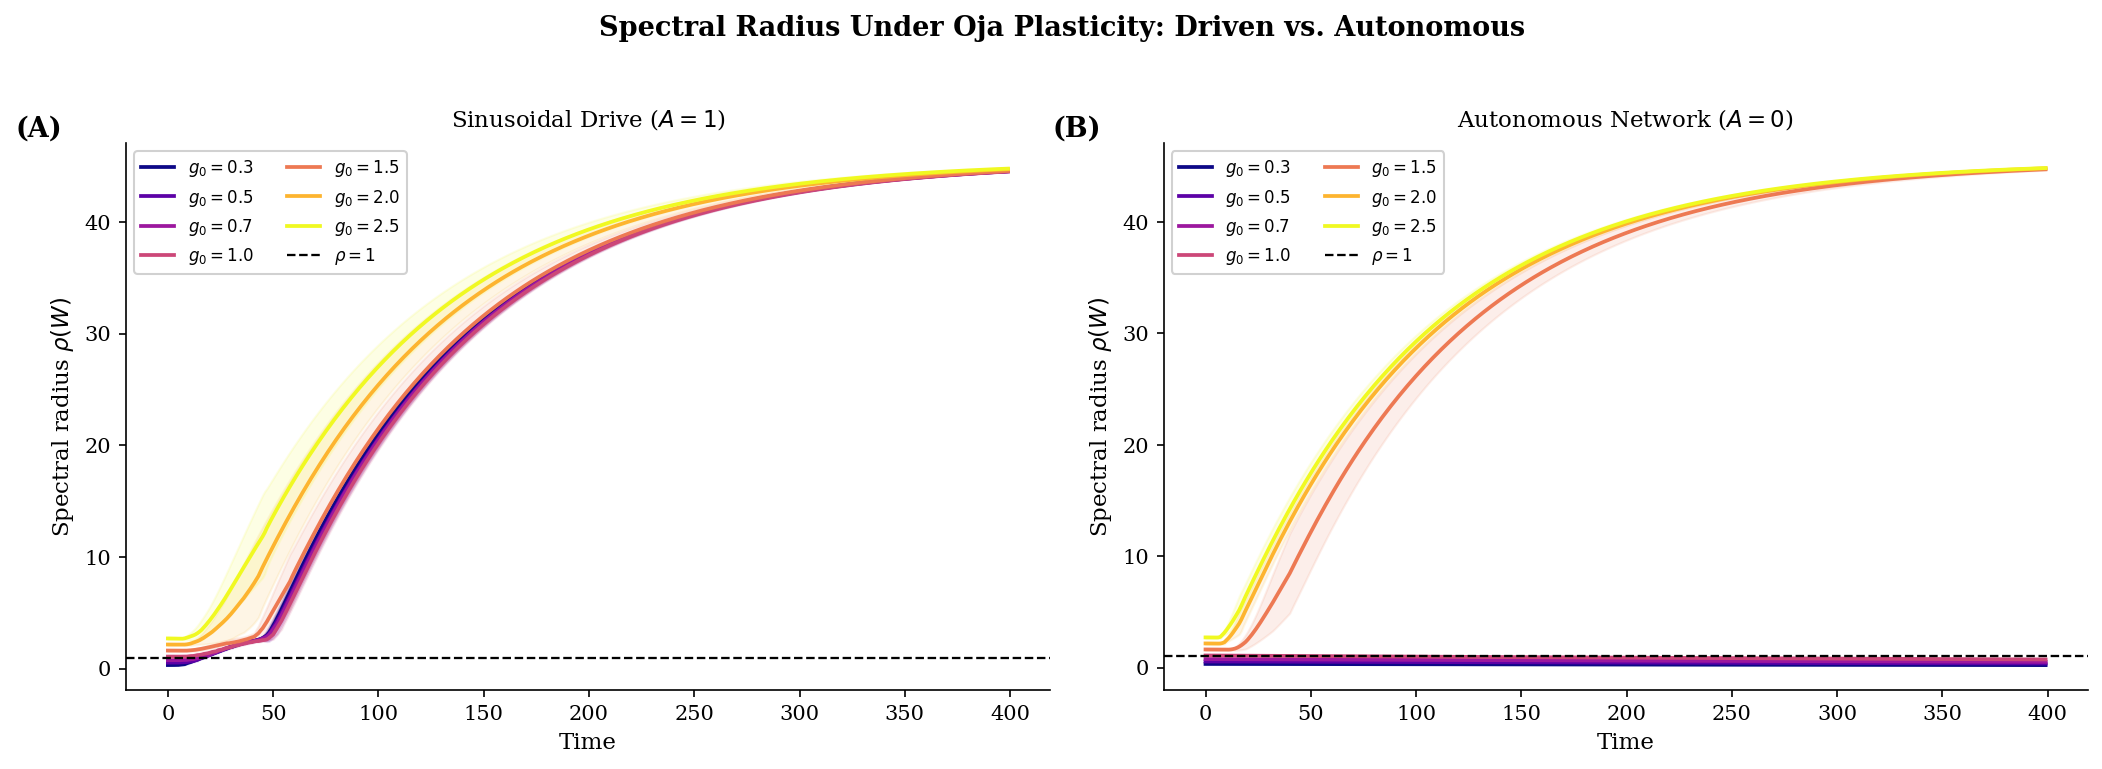
\includegraphics[width=0.75\textwidth]{oja_chaos/spectral_radius_trajectories.png}
    \caption{Spectral radius $\rho(W(t))$ over time for all initial conditions $g_0$
    under sinusoidal drive (left) and autonomous dynamics (right).}
    \label{fig:rho_traj}
\end{figure}
Under sinusoidal drive ($A=1$), the spectral radius of the blows up for all initial conditions ($\rho(W) \to 45$ for every initial $g_0$), with all
trajectories converging within $T \approx 150$ time units (Figure~\ref{fig:rho_traj}).
The drive erases all memory of the initial condition. The autonomous system ($A=0$), on the other hand, exhibits a bifurcation at $g_0 = 1$.

These results suggest that addition of periodic input
erases this bifurcation, removing the stable branch near $\rho(W) = 1$.  The
mechanism reflects the analysis in Section~4.3 where the sinusoidal driver creates a low-rank structure which mutually amplifies the spectral radius until the upper bound imposed by the bounded non-linear activation function is reached. The spectral radius in the numerical simulations approaches $45.455$. This suggests that the $x_i$ indeed saturate to approximately $\pm 1$. The assumption that neural phases align however seems to be weaker, which is likely explained by the non-linear distortion of assumed sinusoidal neural activity. 



\subsection{Edge-of-Chaos Optimality for Signal Reconstruction}

While we find that Oja learning does not maintain the network near the edge of chaos, we expect that the
initial spectral radius $g$ still determines the quality of signal reconstruction
during the early learning transient, before the dimension of the weight matrix collapse. For each $g_0$, we run the driven Oja system
for $T = 80$ time units, ideally long enough for activity transients to decay (since $\tau=1$)
but short enough that Oja has not yet fully saturated the network
($\rho(W) \approx 10$--$20$). We then fit a linear readout to reconstruct
$y(t) = \sin(\omega t)$ from the activity history $X \in \mathbb{R}^{T/dt \times n}$, the idea being that the set of sinusoidal waves serves as a basis for periodic functions:

\begin{equation}
    \mathbf{c}^* = \arg\min_{\mathbf{c}}\,\|X\mathbf{c} - \mathbf{y}\|^2,
    \qquad
    R^2 = 1 - \frac{\|X\mathbf{c}^* - \mathbf{y}\|^2}{\mathrm{Var}(\mathbf{y})}.
\end{equation}

\begin{figure}[H]
    \centering
    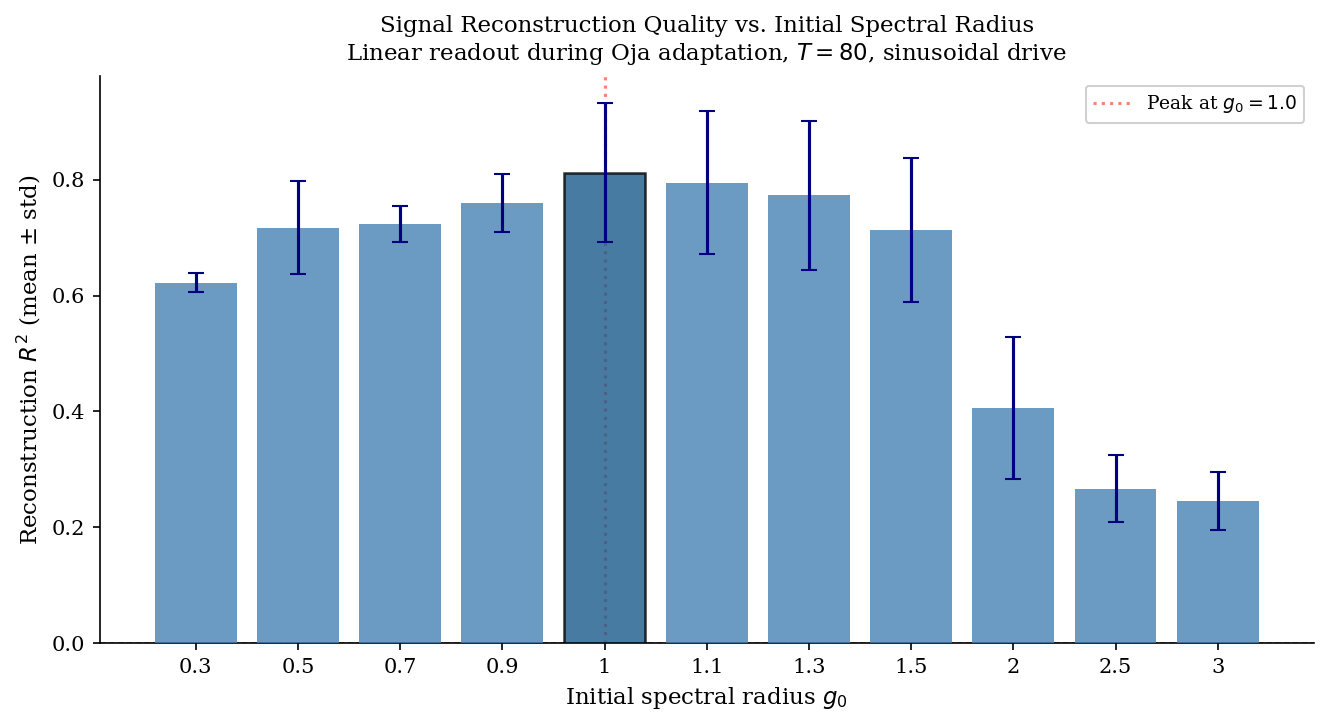
\includegraphics[width=0.7\textwidth]{oja_chaos/r2_vs_g.png}
    \caption{Signal reconstruction $R^2$ as a function of initial spectral radius $g_0$.}
    \label{fig:r2_vs_g}
\end{figure}

$R^2$ peaks at $g_0 \approx 0.9$--$1.0$, reaching $R^2_{\max} \approx 0.81 \pm 0.06$,
and falls to $R^2 \approx 0.22$ at $g_0 = 3.0$ (Figure~\ref{fig:r2_vs_g}).  These results suggest that networks
initialized at the edge of chaos produce the richest activity during the learning
transient, allowing more accurate signal reconstruction before Oja-learning saturates the system, in turn degrading
signal diversity. This is consistent with the theoretical reservoir computing model, where proximity to the edge of chaos maximizes the effective useful dimensionality
of the network's response.

\subsection{Frozen Random Reservoir Outperforms Oja-Learned Weights}

To isolate the degradation of the quality in  signal reconstruction from Oja-type learning, we compare this with a frozen random reservoir.
For each $g_0$, we keep the weights fixed (i.e., $\eta, \lambda = 0$) and fit a ridge-regression
readout with regularization $\alpha = 10^{-3}$. Ridge-regression was used here to account for potential unstable least-squares regression in the high-dimensional, noisy data. 

\begin{equation}
    \mathbf{c}^* = (X^TX + \alpha I)^{-1}X^T \mathbf{y}.
\end{equation}
where $\mathbf{y} = \sin(\omega \mathbf{t})$. 
\begin{figure}[H]
    \centering
    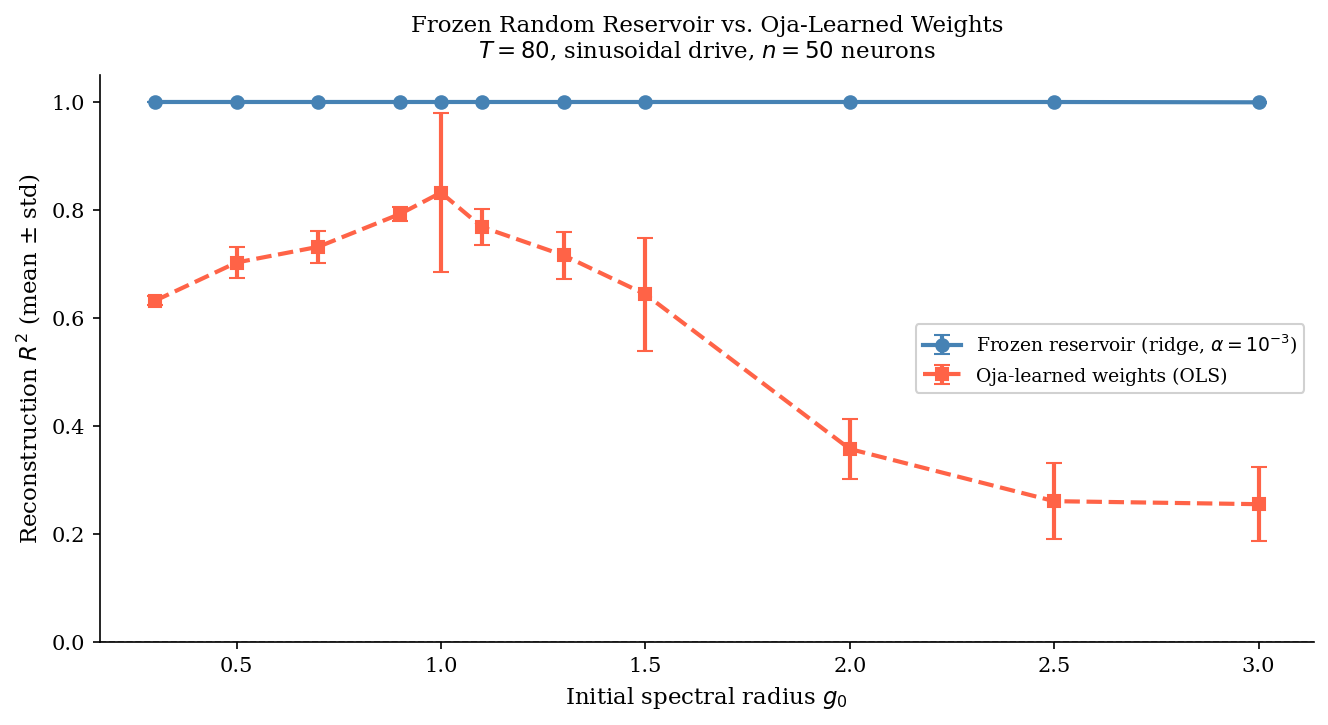
\includegraphics[width=0.7\textwidth]{network_analysis/r2_baseline_vs_oja.png}
    \caption{Comparison of signal reconstruction $R^2$ for Oja-learned weights
    (orange) versus a frozen random reservoir with ridge regression (blue).}
    \label{fig:r2_comparison}
\end{figure}

The frozen reservoir achieves $R^2 \approx 1.0$ for every $g_0$
(Figure~\ref{fig:r2_comparison}). Even this is not a trivial result: the neural network transforms the input sine waves into neural responses with varying amplitude, phases, and nonlinear distortions. On the other hand, Oja-type learning consistently performs worse, driving $\rho(W) \to 45$,
saturating the bounded hyperbolic tangent nonlinearity and degrading the activity diversity in neural activity that allows for high signal reconstruction quality. The frozen network, though, retains useful diversity in neural activity for all $g_0$. \\

\subsection{Input Structure Drives Rank Collapse}

The separation of time scales analysis (Section~4.3) predicts that rank collapse is tied to the
rank of $C(W)$, not to the learning rule itself.  We test this by replacing the
sinusoidal drive with three alternatives:

\begin{itemize}
    \item \emph{Quasi-periodic:} $\frac{A}{\sqrt{3}}\sum_{k=1}^3 \sin(\omega_k t + \phi_i)$,
          with $\omega_1 = 1$, $\omega_2 = \varphi$ (golden ratio), $\omega_3 = \sqrt{2}$
          (chosen to be mutually incommensurate frequencies).
    \item \emph{White noise:} $\xi_i(t) \sim \mathcal{N}(0, A^2/2)$ drawn independently
          for each neuron at each timestep
    \item \emph{Zero drive:} $A = 0$ (autonomous network).
\end{itemize}
The paremeters of each system here were chosen to match $A\sin(\omega t)$ in power, which we use as a proxy for input strength, in order to isolate the effects of the temporal structure on the system (with obvious exception of the autonomous network). 

\begin{figure}[H]
    \centering
    
\includegraphics[width=0.85\textwidth]{signal_comparison/correlation_rank_by_drive.png}
    \caption{Rank of the rolling activity correlation matrix $\hat{C}$ over time for
    all four drive types at $g = 1.0$, using a 2000-step (100 time unit) rolling window.
    Sinusoidal (A) and quasi-periodic (B) drives collapse the rank to 1; white noise (C)
    preserves the full rank $n = 50$; the autonomous network (D) silences to rank~0.}
    \label{fig:rank_collapse}
\end{figure}

Here, we use a 2000-step (100 time unit) rolling window to allow initial transients to settle and to provide enough independent samples for rank estimation to reflect the true signal dimensionality. The results reveal a clear pattern across all four drive types (Figure~\ref{fig:rank_collapse}).  Sinusoidal drive collapses $\mathrm{rank}(\hat{C}) \to 1$ within $T \approx 100$ time units (panel A).
Quasi-periodic drive with three mutually incommensurate frequencies produces nearly
identical collapse, reaching $\mathrm{rank}(\hat{C}) \approx 1$ by $T \approx 150$
time units (panel B).  Both structured drives push $\rho(W) \to 43$ regardless of
initial spectral radius.

White noise preserves full-rank correlations: $\mathrm{rank}(\hat{C}) \to n = 50$ in
steady state (panel C).  The isotropic structure of white noise gives
$C \approx \sigma^2 I$, so $W^* \approx (\eta\sigma^2/\lambda) I$ is full-rank with
bounded spectral radius.  In the autonomous case ($A = 0$, panel D), the network
silences at $g = 1$: without external drive, the stable fixed point at the origin
dominates, yielding $\mathrm{rank}(\hat{C}) \to 0$.

These results confirm that rank collapse is driven by the temporal structure of the
input, not by Oja learning alone.  The quasi-periodic result is particularly striking:
three mutually incommensurate frequencies are still insufficient to prevent collapse.
The crucial distinction is not the number of active spectral modes but whether the
input correlation matrix $C$ has low rank---any finite set of periodic components
produces a finite-rank $C$ that Oja then amplifies to drive $\rho(W) \to 45$.


\subsection{Effective Gain Is Self-Regulated by Saturation}

In this section, we seek to validate the heuristic effective gain in two complementary experiments. 

In the first experiment, we track $g_{\mathrm{eff}}(t)$ during Oja learning alongside $\rho(W(t))$ for sinusoidal and white noise drives. \hl{At each simulation step $g_{\mathrm{eff}}$ is computed from the current pre-activations $h_i = [Wx]_i$ and the Frobenius norm of $W$ using the heuristic formula above.} Under sinusoidal drive, we find that $\rho(W)$ approaches approximately $43$ but every neuron saturates ($|h_i| \to \infty$), so
$d_i = \operatorname{sech}^2(h_i) \to 0$ and $g_{\mathrm{eff}} \to 0$.  Here, the system is in a maximally saturated state where the linearized perturbation dynamics
 are always stable despite the exploding nominal spectral radius.

In our second experiment, \hl{weights are frozen ($\eta, \lambda = 0$) to isolate the $D(t)W$ contribution to stability from the Oja weight dynamics.} We scan $g \in [0.1, 3.0]$ with sinusoidal drive, averaging $g_{\mathrm{eff}}$ and $\rho(D(t)W)$ over the steady-state window $t \in [210, 300]$.

\begin{figure}[H]
    \centering
    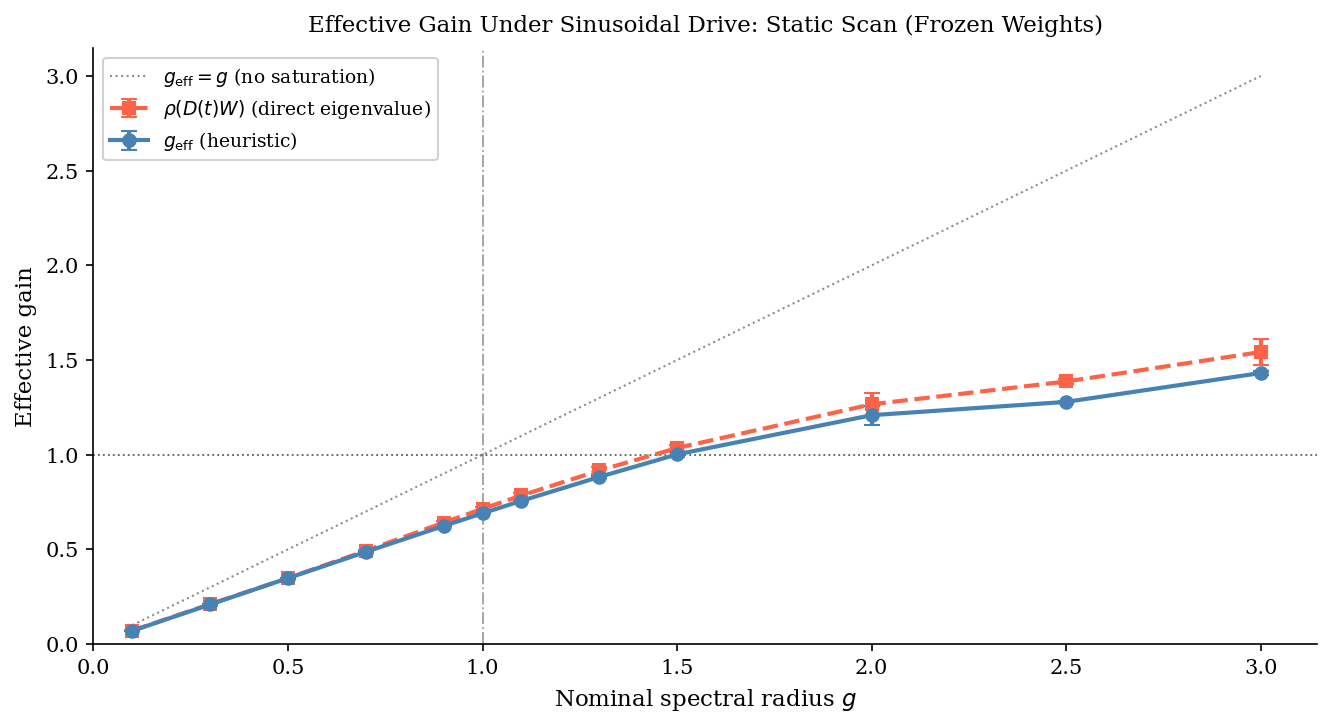
\includegraphics[width=0.7\textwidth]{geff/geff_static_scan.png}
    \caption{Time-averaged effective gain $g_{\mathrm{eff}}$ (blue) and directly calculated spectral radius
    $\rho(D(t)W)$ (orange) versus nominal $g$ for frozen weights under sinusoidal
    drive. The dotted diagonal shows the no-saturation baseline $g_{\mathrm{eff}} = g$.}
    \label{fig:geff_scan}
\end{figure}

Here we see that the heuristic tracks the effective spectral radius $\rho(D(t)W)$ within 5\% across all tested $g$ (Figure~\ref{fig:geff_scan}).  The $g_{\mathrm{eff}} = 1$ crossing occurs at $g \approx 1.5$: sinusoidal drive saturates neurons enough to reduce the effective gain by approximately 33\%, shifting the effective stability boundary substantially above the Girko prediction $g = 1$. \hl{Here $g$ is the nominal distribution parameter used to initialize the weight matrix, i.e.\ $W_{ij}\sim\mathcal{N}(0,g^2/n)$; by Girko's circular law $\rho(W)\approx g$ for large $n$, though at $n=50$ a finite-size gap is present.}


\subsection{Critical Slowing Down at the Phase Transition}

Independent evidence for the $g = 1$ phase transition comes from the autonomous
discrete map $h_{t+1} = Wf(h_t)$.  The largest Lyapunov exponent (LLE) $\lambda_1$
is estimated via a 300-step warmup followed by 800-step single-vector power iteration
on the tangent map $J_t = W\operatorname{diag}(\operatorname{sech}^2(h_t))$.  For
$\lambda_1 < 0$ the system is stable with relaxation time
$\tau_{\mathrm{relax}} = -1/\lambda_1$; for $\lambda_1 > 0$ the map is chaotic.
In the linear regime a small perturbation $\delta h(0)$ is predicted to grow as
$\|\delta h(t)\| \approx \varepsilon\,e^{\lambda_1 t}$.

\begin{figure}[H]
    \centering
    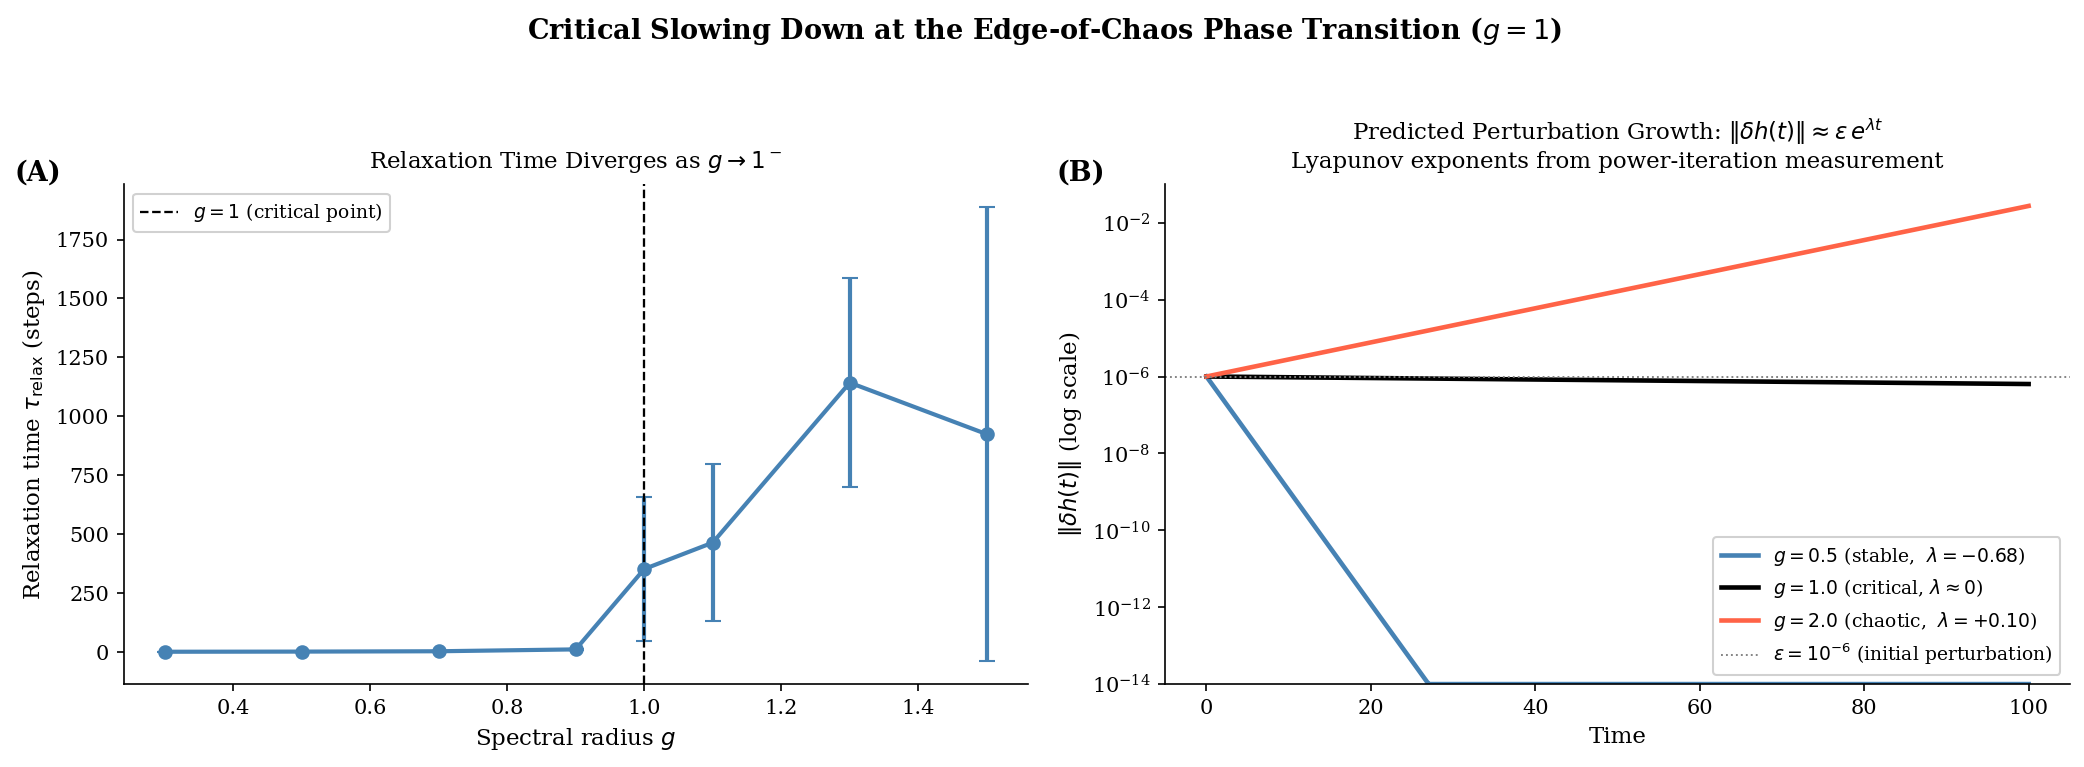
\includegraphics[width=0.85\textwidth]{network_analysis/critical_slowing_down.png}
    \caption{Left: relaxation time $\tau_{\mathrm{relax}} = -1/\lambda_1$ versus $g$
    for the autonomous discrete map; $\tau_{\mathrm{relax}}$ diverges as $g \to 1^-$.
    Right: predicted perturbation growth $\|\delta h(t)\| = \varepsilon\,e^{\lambda_1 t}$
    using the power-iteration LLE values, illustrating the stable ($g = 0.5$), critical
    ($g = 1.0$), and chaotic ($g = 2.0$) regimes.}
    \label{fig:csd}
\end{figure}

\begin{table}[h]
    \centering
    \caption{Largest Lyapunov exponent and relaxation time for selected $g$ values
    ($n = 50$, autonomous discrete map, mean over 5 seeds).}
    \label{tab:lle}
    \begin{tabular}{lrr}
    \toprule
    $g$ & $\lambda_1$ (nats/step) & $\tau_{\mathrm{relax}}$ (steps) \\
    \midrule
    $0.30$ & $-1.20$ & $0.8$ \\
    $0.70$ & $-0.35$ & $2.9$ \\
    $0.90$ & $-0.10$ & $10.8$ \\
    $1.00$ & $-0.005$ & $\approx 350$ \\
    $2.00$ & $+0.10$  & (chaotic) \\
    \bottomrule
    \end{tabular}
\end{table}

Table~\ref{tab:lle} and Figure~\ref{fig:csd} show that $\tau_{\mathrm{relax}}$
diverges as $g \to 1^-$, which is the defining signature of a continuous (second-order)
phase transition \cite{guckenheimer1983nonlinear}.  At $g = 1$ the network has no
preferred timescale for returning to equilibrium: small disturbances persist
arbitrarily long.  This critical slowing down provides a physically clean signature
of the edge-of-chaos transition that is observable independently of the sign of the
LLE.

A note on finite-size effects: Sompolinsky's mean-field theory \cite{sompolinsky1988chaos}
predicts chaos onset exactly at $g = 1$ in the $n \to \infty$ limit.  For $n = 50$,
the discrete map remains stable up to $g \approx 1.5$ (LLE $\approx -0.009$); positive
LLE first appears near $g \approx 2.0$ (Table~\ref{tab:lle}).  The $\tau_{\mathrm{relax}}$
divergence near $g = 1$ is nonetheless clearly visible and confirms the qualitative
picture even at finite $n$.

\hl{A natural question is why $\tau_{\mathrm{relax}}$ diverges at $g = 1$ here, while the effective-gain analysis (Section~5.5) found $g_{\mathrm{eff}} = 1$ only at $g \approx 1.5$. The reconciliation is that these two experiments probe different dynamical regimes. The critical slowing down experiment uses the autonomous network ($A = 0$), initialized with small activity. Without external drive, neurons remain near the origin, so $h_i \approx 0$ and $d_i = \operatorname{sech}^2(h_i) \approx 1$ for all $i$. The effective gain therefore reduces to $g_{\mathrm{eff}} \approx g$, and the edge-of-chaos transition occurs exactly at $g = 1$ in agreement with Girko's law. By contrast, sinusoidal drive (Section~5.5) saturates neurons ($|h_i| \gg 1$, $d_i \ll 1$), pulling $g_{\mathrm{eff}}$ well below $g$. The effective stability boundary is thereby shifted upward to $g \approx 1.5$. In short, neural saturation induced by structured input is what displaces the effective chaos onset; in the unsaturated autonomous case, $g_{\mathrm{eff}} = g$ and the classical $g = 1$ threshold is recovered.}



\section{Conclusions}
Weight matrix structure determines system behavior, in terms of both neural activity and the network's computational power. From the analysis of the non-driven autonomous network, we found that nontrivial behavior that asymptotically tend to the equilibrium, but can still exhibit complex, high-dimensional transient dynamics, only exists near the "edge of chaos", where the system is between the parameter regions of stability and instability. For random matrices, having effective gain near $1$ gives the highest likelihood of the system operating near the edge of chaos and exhibiting the behavior necessary for signal reconstruction and computation.
\vspace{0.5cm}
\\
Additionally, we explored how "random modes" through reservoir computing provide a basis for computation, which relies on high-dimensional structure preserved by pseudo-random input. Oja-type plasticity reduces dimensionality of the weight matrix depending on dimensionality of the inputs, which can reduce the computational power of the network. Stated differently, Oja-type plasticity combined with structured inputs induces low-rank synchronization, which can suppress the high-dimensional transient diversity required for reservoir-type computation. This qualitatively resembles the abnormal synchronization observed in seizure-like neural activity in epilepsy patients.
%----------------------------------------------------------------------------------------
%	REFERENCES 
%----------------------------------------------------------------------------------------
\clearpage
\nocite{*}
\bibliographystyle{plain}
\bibliography{references}


\end{document}